\chapter{Appendix B}

\section{Additional Apparatus Pictures} \label{sec:additional_apparatus}

\begin{figure}[htpb]
    \centering
    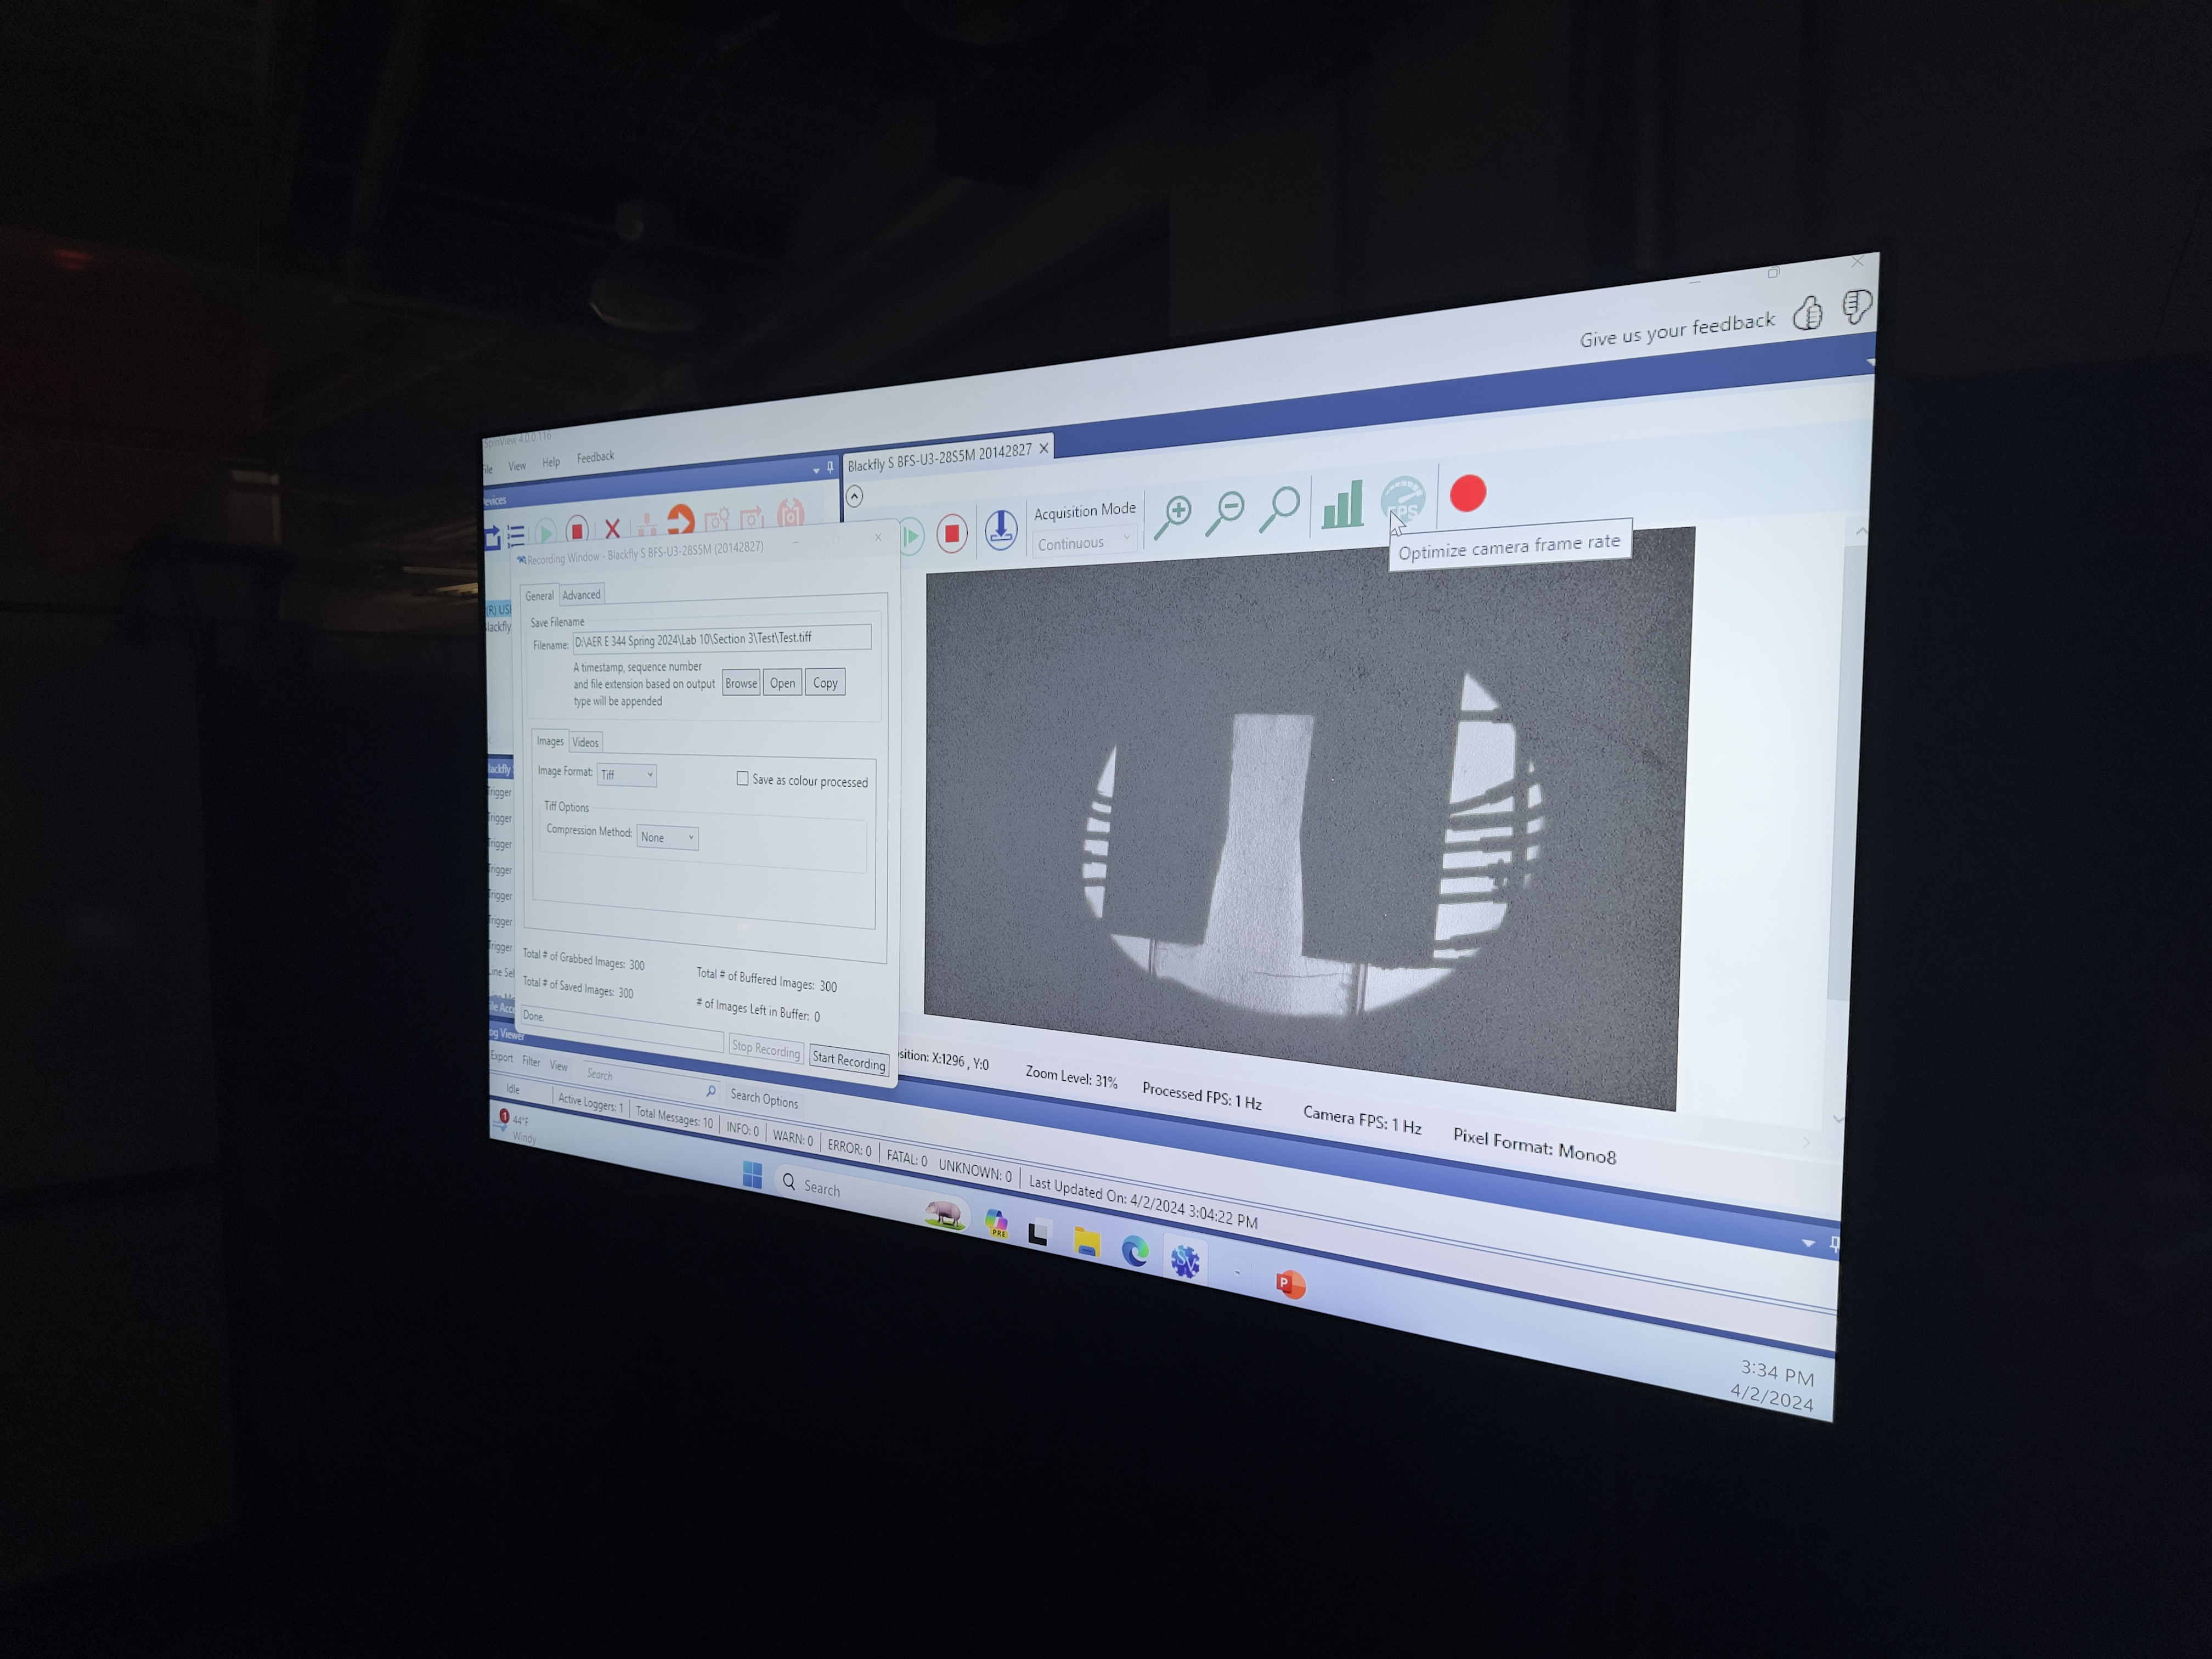
\includegraphics[width=0.75\linewidth]{Figures/camera_capture_settings.jpeg}
    \caption{The settings for the camera in the Schlieren setup.}
    \label{fig:camera_settings}
\end{figure}

\begin{figure}[htpb]
    \centering
    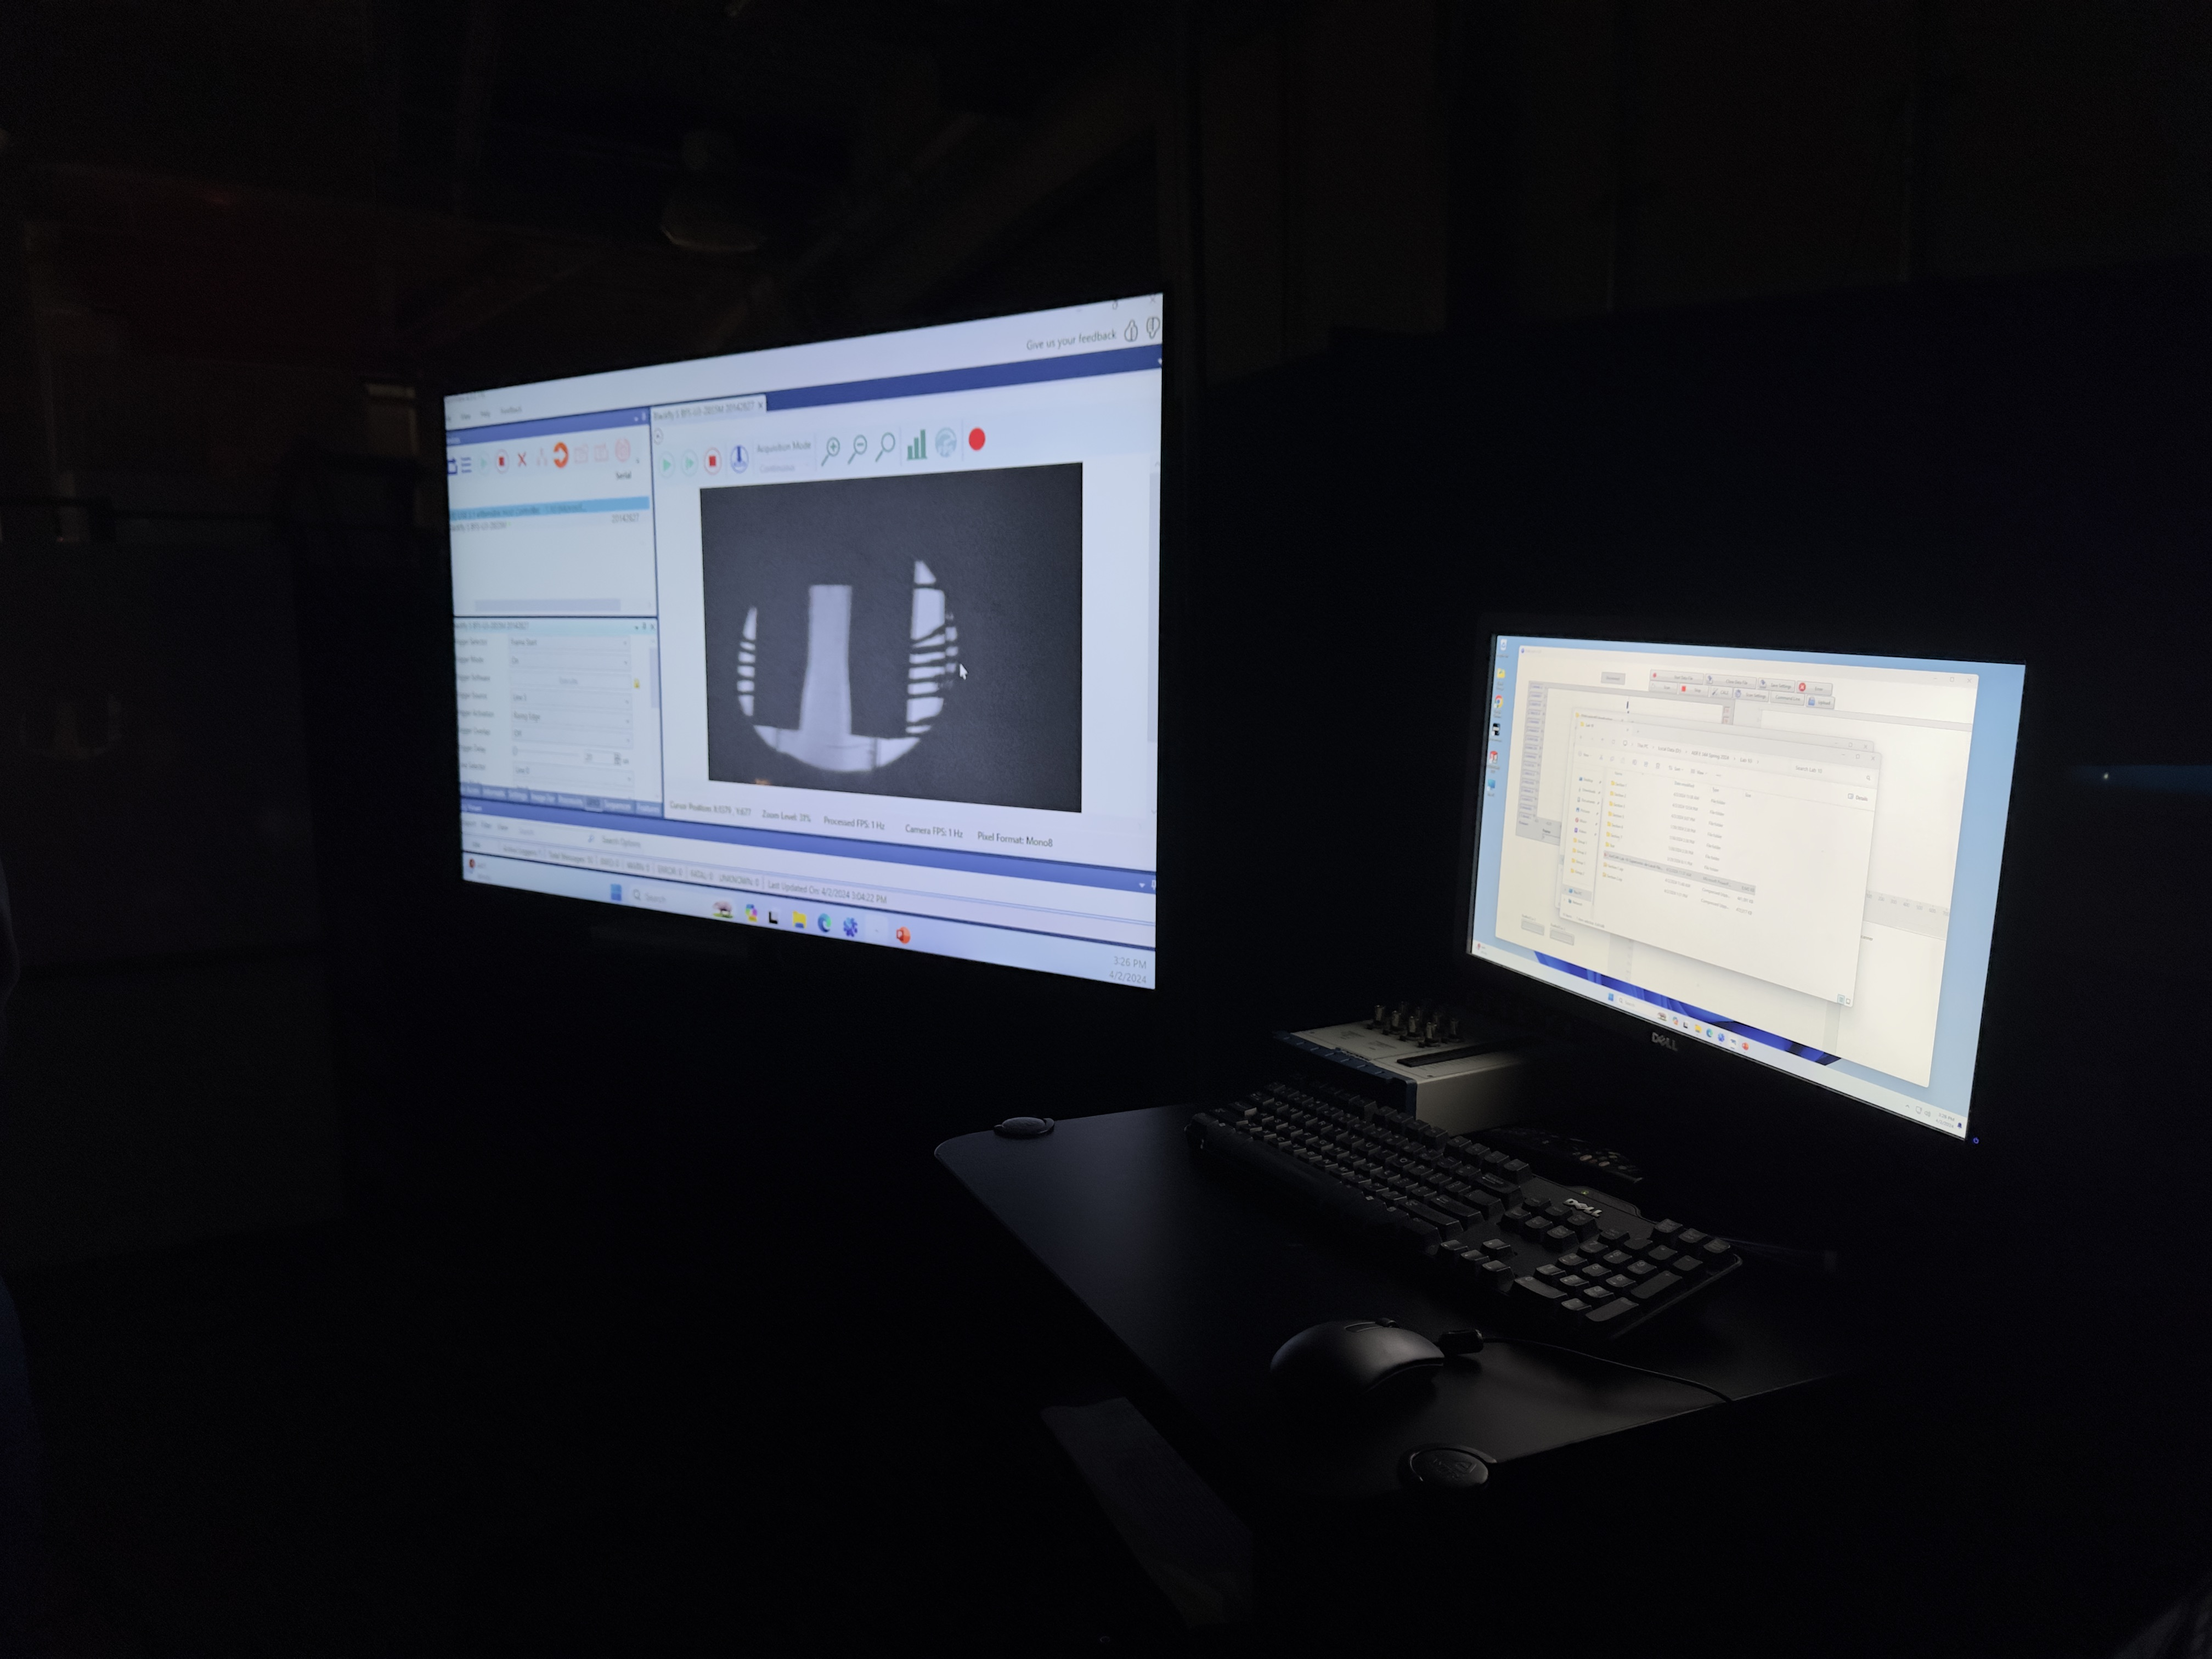
\includegraphics[width=0.75\linewidth]{Figures/data_acquisition_software.jpeg}
    \caption{The data acquisition software and the image capture software.}
    \label{fig:data_acquisition}
\end{figure}

\begin{figure}[htpb]
    \centering
    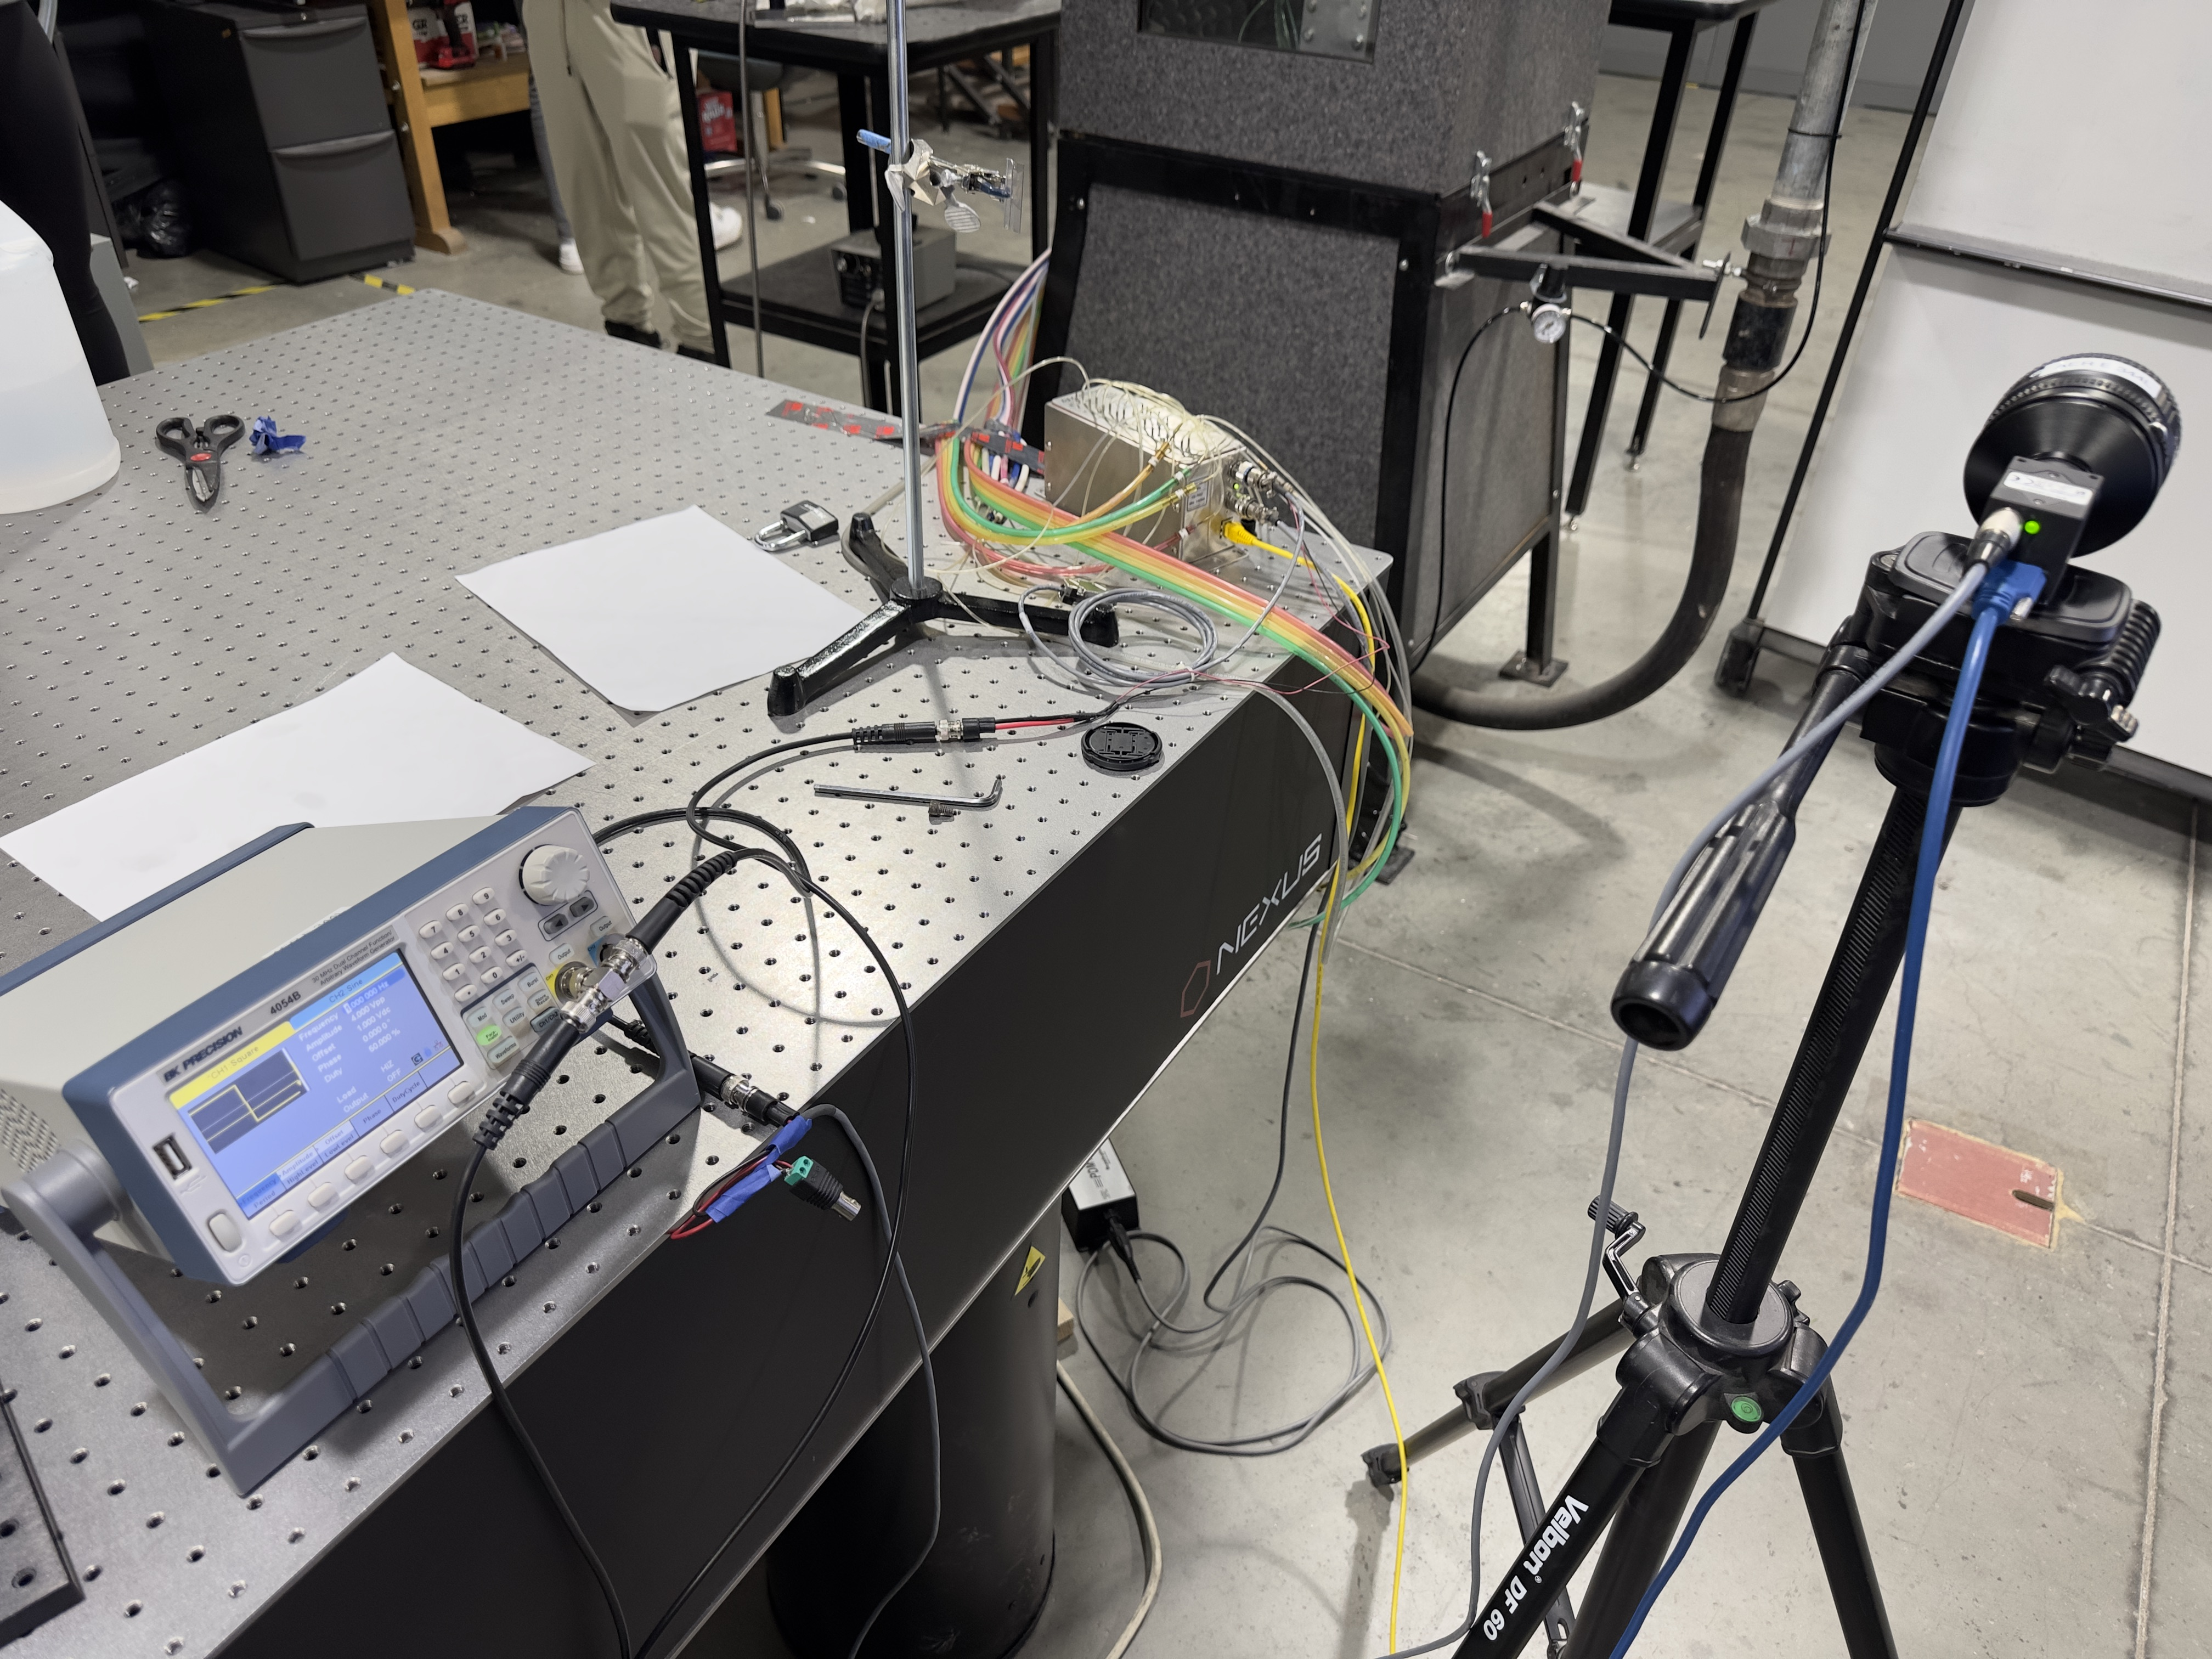
\includegraphics[width=0.75\linewidth]{Figures/delay_generator_and_schlieren.jpeg}
    \caption{The camera, delay generator, and the pressure transducer.}
    \label{fig:delay_generator}
\end{figure}

\begin{figure}[htpb]
    \centering
    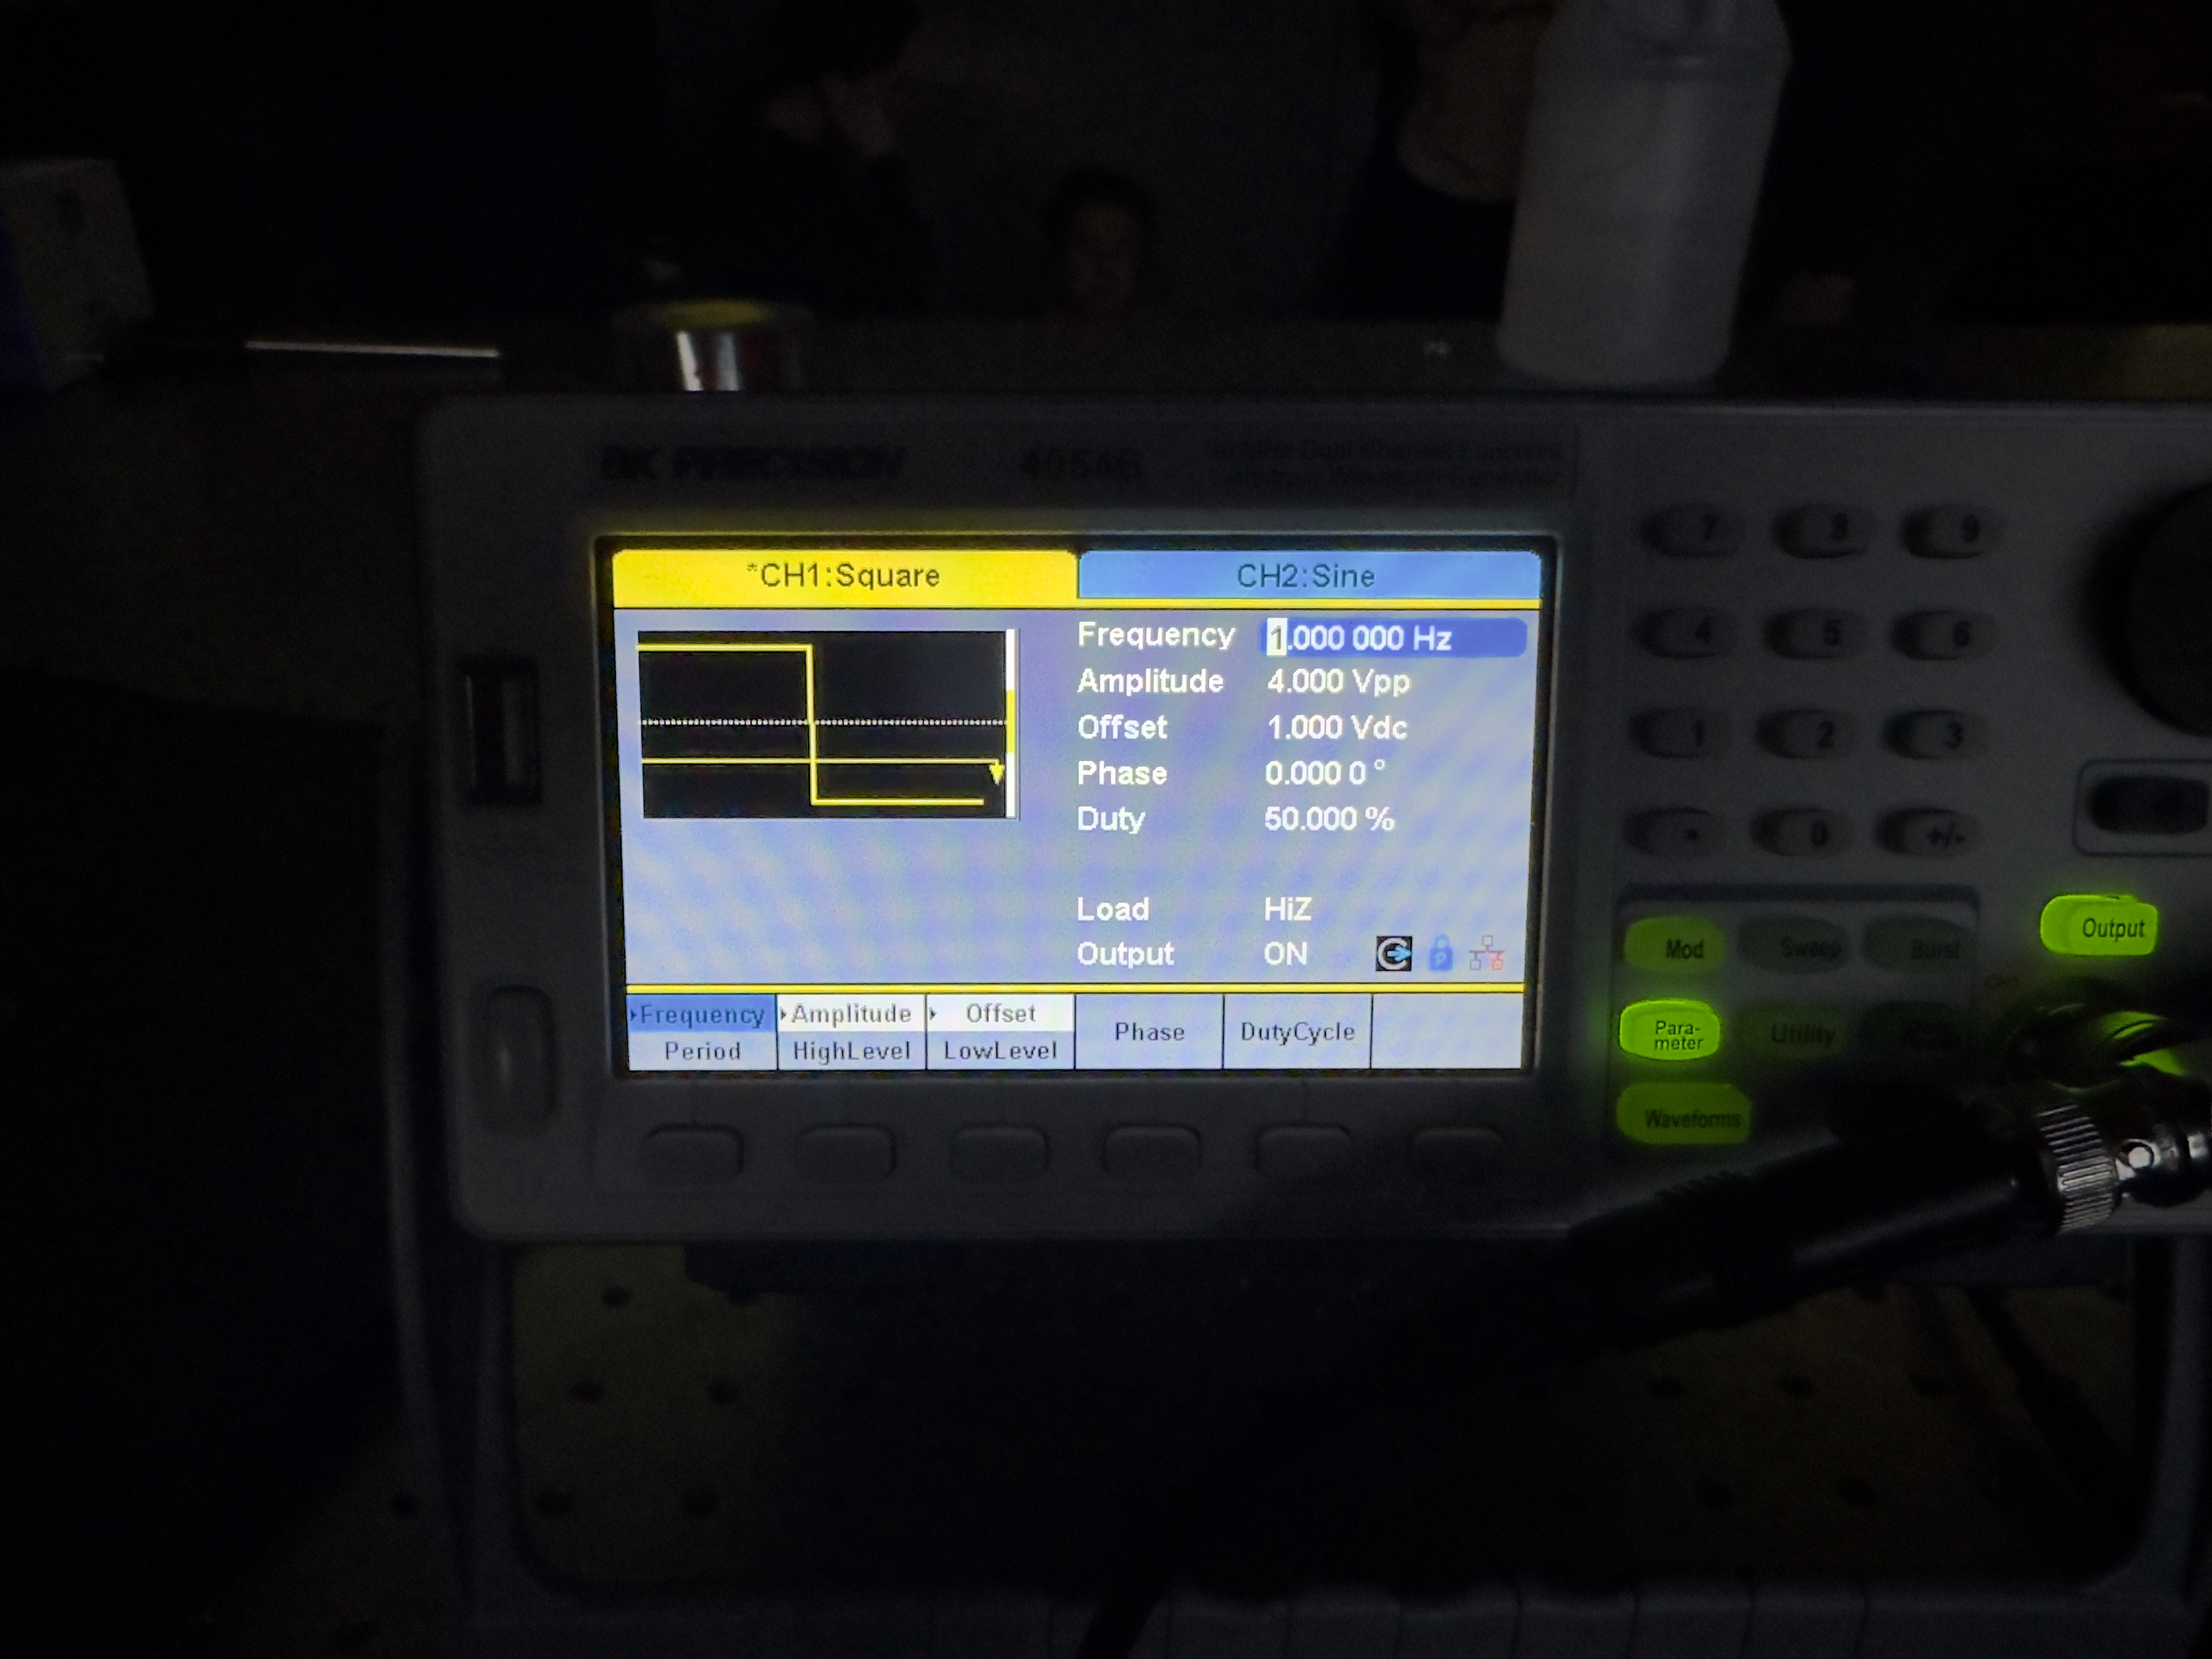
\includegraphics[width=0.75\linewidth]{Figures/delay_generator_settings.jpeg}
    \caption{The settings for the delay generator.}
    \label{fig:delay_generator_settings}
\end{figure}

\begin{figure}[htpb]
    \centering
    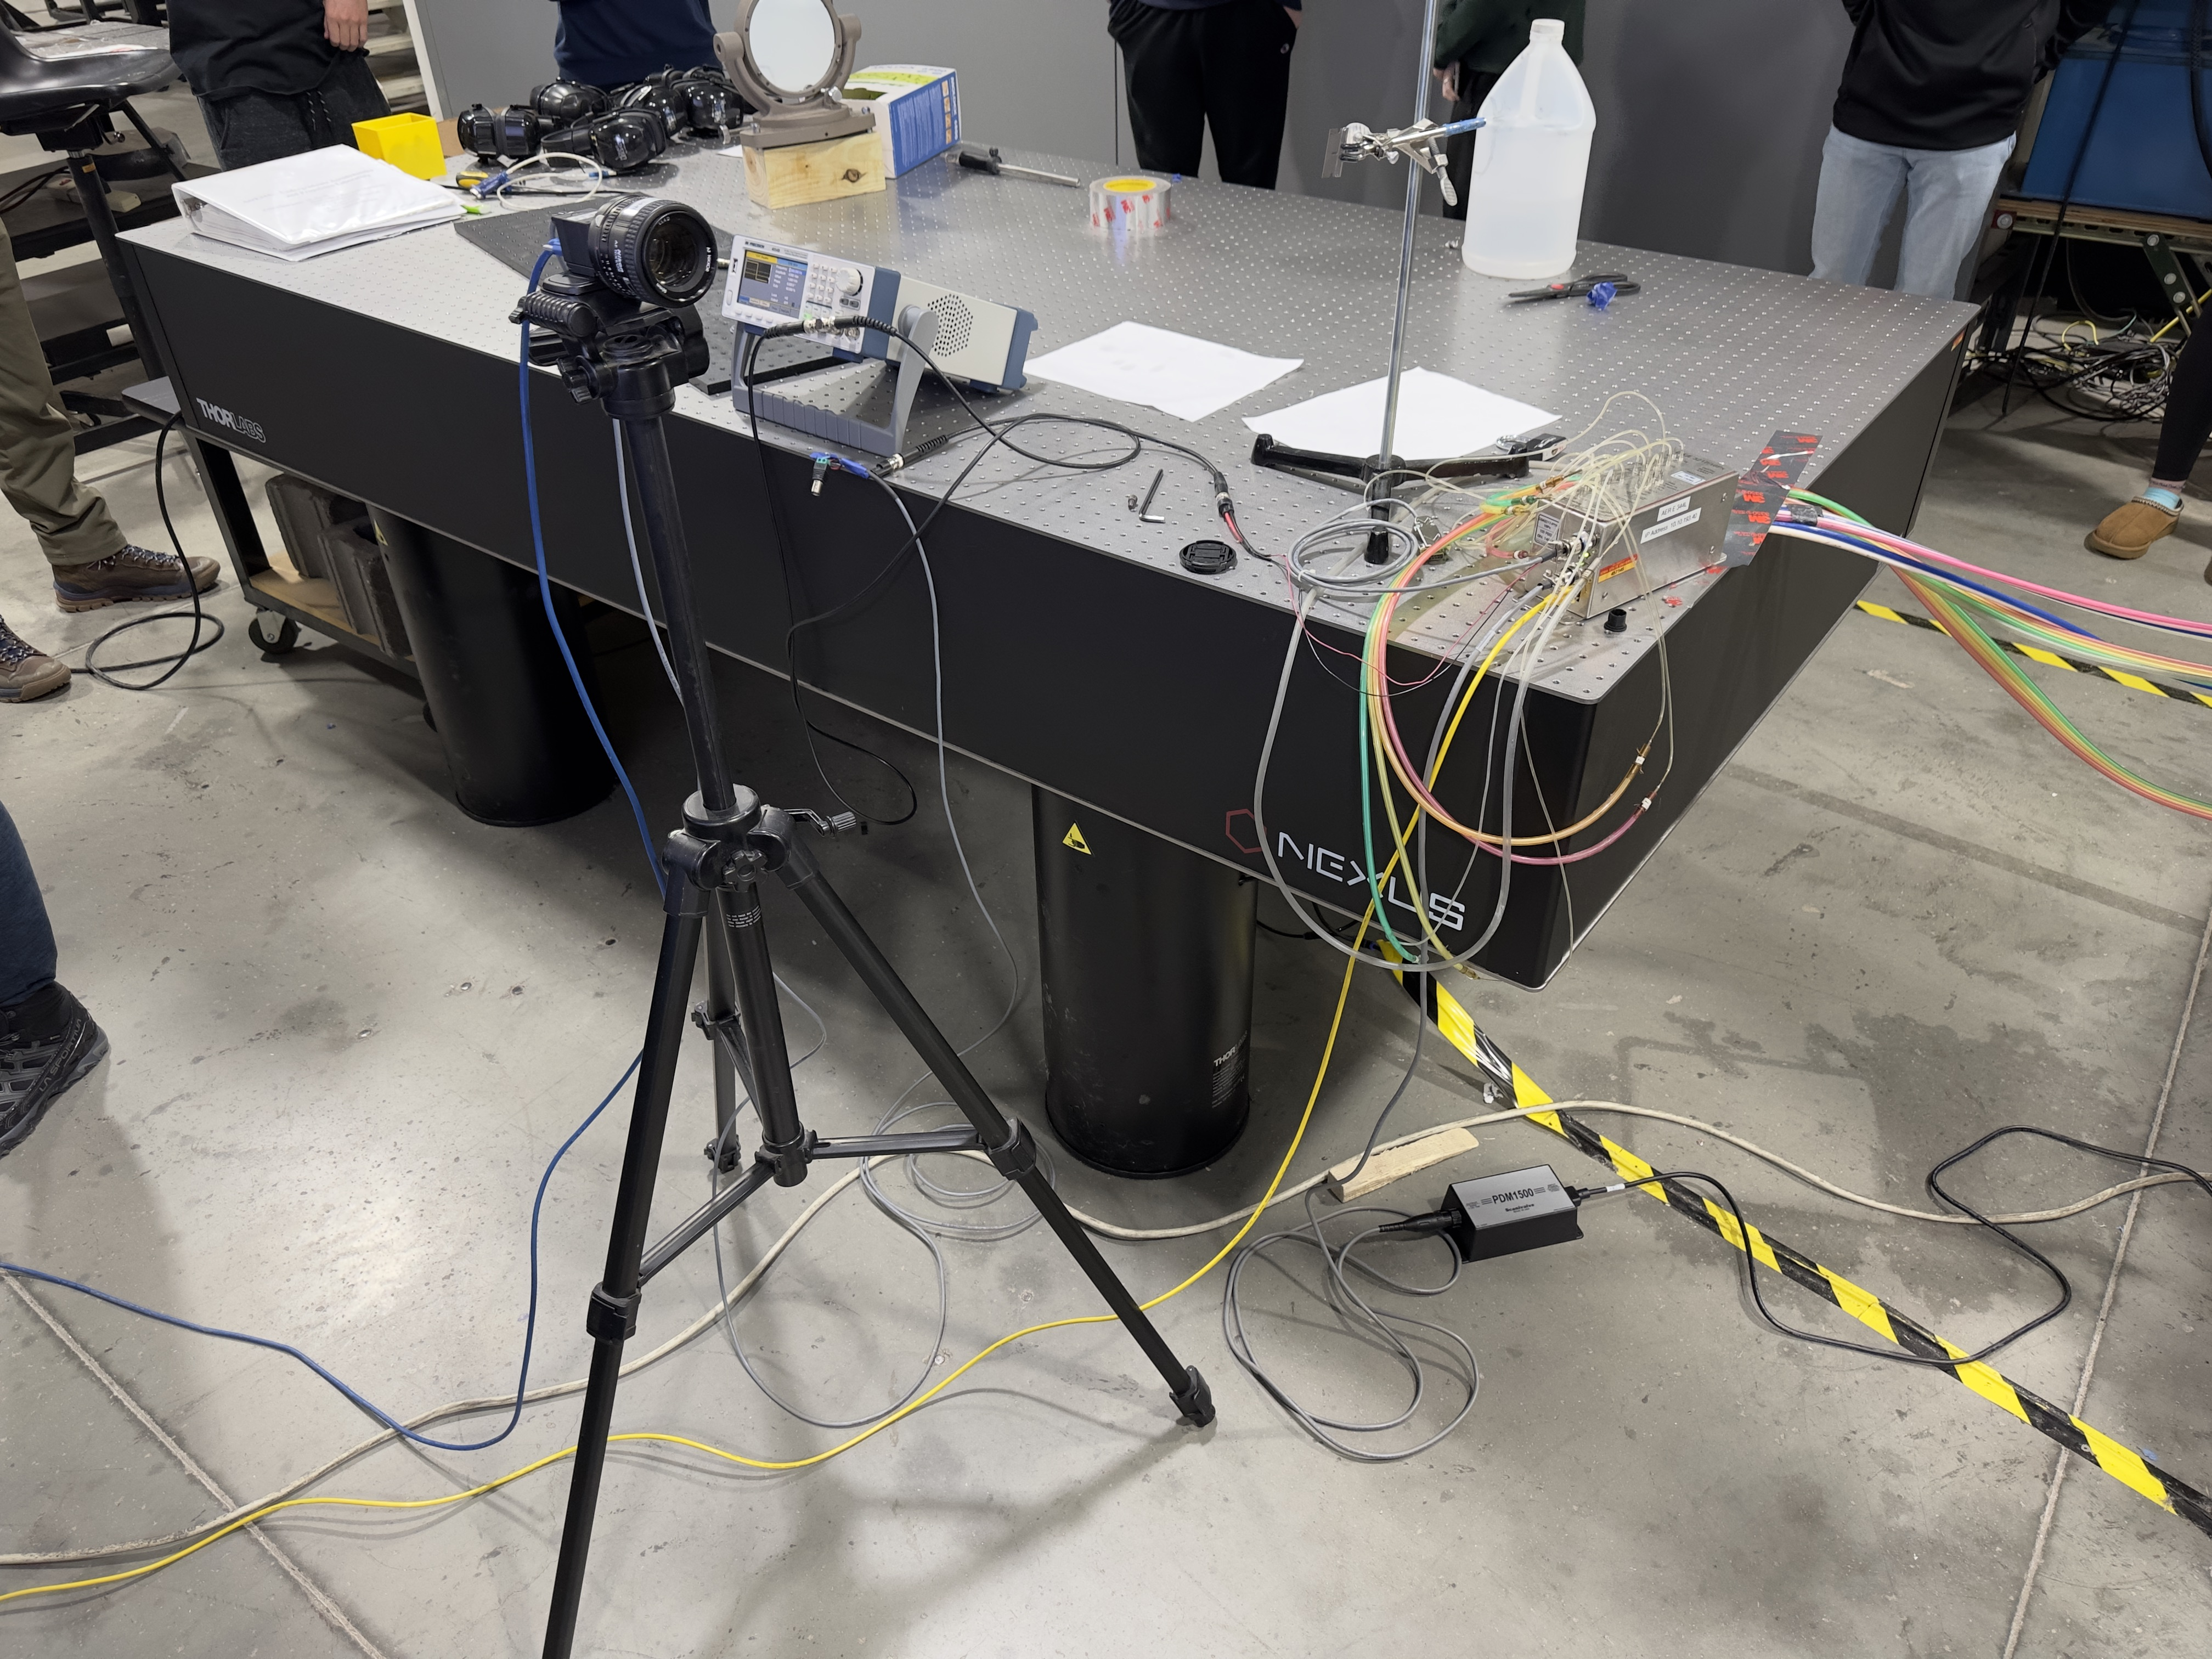
\includegraphics[width=0.75\linewidth]{Figures/camera.jpeg}
    \caption{The camera in the Schlieren configuration takes high-contrast images of the projections of flow passing through the de Laval nozzle.}
    \label{fig:camera}
\end{figure}

\newpage

\section{Additional Figures} \label{sec:additional_figures}

\begin{figure}[htpb]
    \centering
    \includesvg[width=0.75\linewidth]{Figures/Measured Pressure Distribution - 1st Critical Condition.svg}
    \caption{A plot of the measured pressure distribution in the de Laval nozzle when the flow is at the first critical condition.}
    \label{fig:measured_pressure_1st_critical}
\end{figure}

\begin{figure}[htpb]
    \centering
    \includesvg[width=0.75\linewidth]{Figures/Measured Pressure Distribution - Normal Shock Inside the Nozzle.svg}
    \caption{A plot of the measured pressure distribution in the de Laval nozzle when the flow has a normal shock in the divergent section of the nozzle.}
    \label{fig:measured_pressure_normal_shock}
\end{figure}

\begin{figure}[htpb]
    \centering
    \includesvg[width=0.75\linewidth]{Figures/Measured Pressure Distribution - 2nd Critical Condition.svg}
    \caption{A plot of the measured pressure distribution in the de Laval nozzle when the flow is at the second critical condition.}
    \label{fig:measured_pressure_2nd_critical}
\end{figure}

\begin{figure}[htpb]
    \centering
    \includesvg[width=0.75\linewidth]{Figures/Measured Pressure Distribution - 3rd Critical Condition.svg}
    \caption{A plot of the measured pressure distribution in the de Laval nozzle when the flow is at the third critical condition.}
    \label{fig:measured_pressure_3rd_critical}
\end{figure}

\begin{figure}[htpb]
    \centering
    \includesvg[width=0.75\linewidth]{Figures/Theoretical Pressure Distribution - 1st Critical Condition.svg}
    \caption{A plot of the theoretical pressure distribution in the de Laval nozzle when the flow is at the first critical condition.}
    \label{fig:theoretical_pressure_1st_critical}
\end{figure}

\begin{figure}[htpb]
    \centering
    \includesvg[width=0.75\linewidth]{Figures/Theoretical Pressure Distribution - Normal Shock Inside the Nozzle.svg}
    \caption{A plot of the theoretical pressure distribution in the de Laval nozzle when the flow has a normal shock in the divergent section of the nozzle.}
    \label{fig:theoretical_pressure_normal_shock}
\end{figure}


\begin{figure}[htpb]
    \centering
    \includesvg[width=0.75\linewidth]{Figures/Theoretical Pressure Distribution - 2nd Critical Condition.svg}
    \caption{A plot of the theoretical pressure distribution in the de Laval nozzle when the flow is at the second critical condition.}
    \label{fig:theoretical_pressure_2nd_critical}
\end{figure}

\begin{figure}[htpb]
    \centering
    \includesvg[width=0.75\linewidth]{Figures/Theoretical Pressure Distribution - 3rd Critical Condition.svg}
    \caption{A plot of the theoretical pressure distribution in the de Laval nozzle when the flow is at the third critical condition.}
    \label{fig:theoretical_pressure_3rd_critical}
    \vspace*{5.5in}
\end{figure}
